% #############################################################################
% This is Chapter 3
% !TEX root = ../main.tex
% #############################################################################
% Change the Name of the Chapter i the following line
\fancychapter{Case Study: Don't Starve Together}
\cleardoublepage
% The following line allows to ref this chapter
\label{chapter:case-study-dst}

\noindent Don't Starve Together is a multiplayer wilderness survival game developed by Klei Entertainment, where the players must survive as long as they can.
The players must face the harshnesses of a procedurally generated world that is actively trying to kill them, either by cooperating or competing with each other.
Each game can last an indefinite amount of time which is only determined by the players' ability to survive: the better you play the game, the longer you can last.

Released on April 21st of 2016, \ac{DST} is the standalone multiplayer expansion of the uncompromising wilderness survival game Don't Starve, also released by Klei on April 23rd of 2013 (check Fig. \ref{fig:don't-starve-together-poster}).
Both titles are available in several platforms ranging from PC's to consoles and even mobile devices.
By the end of 2013 the original title (Don't Starve) sold over one million copies and, currently, there are almost 3.5 million owners of the game only on Steam.
\ac{DST} counts with over 7 million owners on Steam and has a daily peak of concurrent players of about 8 thousand, reaching as high as 12 thousand concurrent players.

\begin{figure}
  \centering
  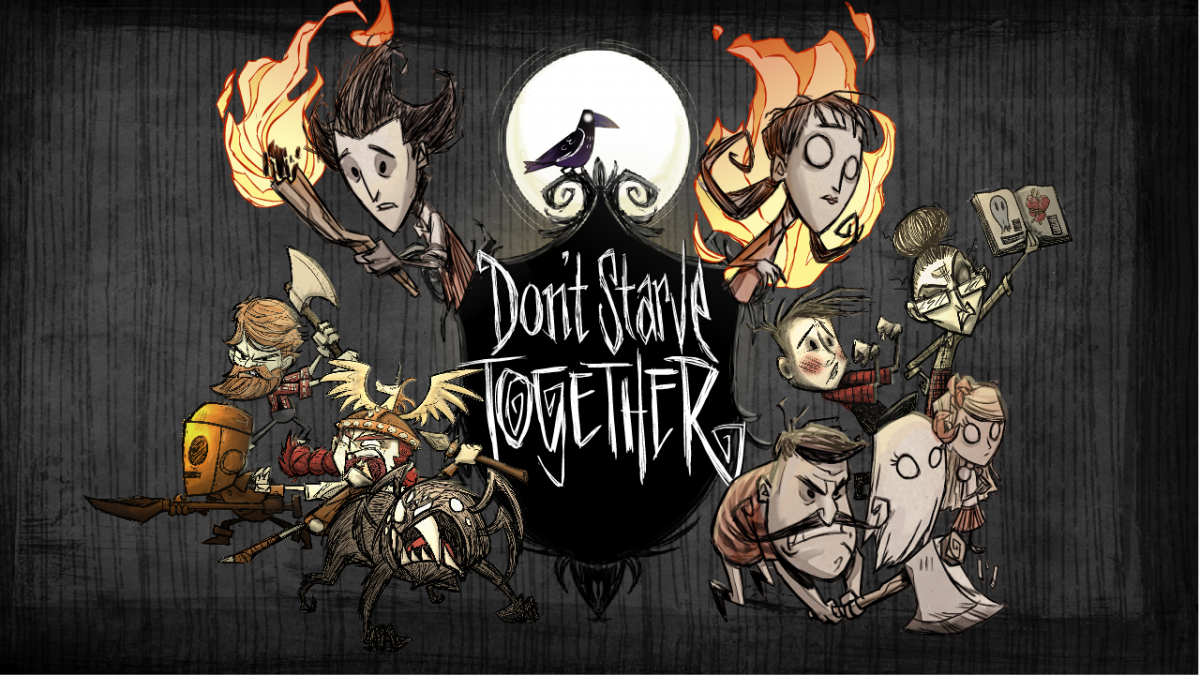
\includegraphics[width=\textwidth]{./Images/dont-starve-together-poster}
  \caption{Don't Starve Together poster with all original characters.}
  \label{fig:don't-starve-together-poster}
\end{figure}

The game counts with a developer maintained forum where there is an active participation by Klei Entertainment staff, which help in problem solving for community developed mods, bug fixing the game, and sharing development notes on the game.
Currently, over five thousand mods are available for the game on the Steam Workshop.

As we've previously discussed, survival games offer players different challenges that must be overcome by the character in order to survive.
Some do it by providing mechanics for hunger and thirst while others provide horrific scenarios like zombie infested worlds.

\ac{DST} borrows ideas from both sides.
The game presents mechanics for hunger, health, temperature, wetness, day and night cycles, seasons, and sanity.
It also provides players with a monster infested world that try to kill the player's character.
The addition of multiplayer brings the possibility for social interaction among players, which contributes positively for the gameplay experience.

Moreover, the sanity mechanic itself is a differentiating factor from other games in the genre.
By providing a measurement of the characters' mental health, the game makes the characters more human and relatable.
A normal human being under such harsh environments would suffer physically but also mentally, and the sanity mechanic depicts just that.

For these reasons, the lack of \ac{AI} controlled \acp{NPC} with believable behaviour, the ability to control and personalize the generated game world, and the possibility of introducing modifications into the game, we've decided to use this game as the target of our project.

For the remainder of this chapter we will present a thorough break down of the game.
We'll explain what the game consists in and move on to describing the game's world.
Then, a general gameplay experience is briefly described before ending the chapter with a summarization of the game mechanics.

\section{The Game}

\noindent Before playing \ac{DST}, the player must first generate a game world to play in.
The generation process will create a new world in accordance to a set of configurations.
The configurations allows her to personalize every aspect of the game world, including the world size, the abundance of resources, the existence and frequency of monster appearances, and many more options.

The player will then choose a character from a list of available characters.
Different characters have different characteristics and may be affected by the world in different ways (for example, WX-78 can eat spoiled food without penalties) and can even possess special items (such as Woodie's axe, \textit{Lucy the Axe}).
Upon entering the world, the player has nothing in its inventory (except for character specific items) and thus needs to start collecting resources in order to survive.

During the game, the player must pay attention to the three characteristics of her character: Hunger, Sanity, and Health.
The player dies (in \ac{DST} the player actually becomes a ghost that can be revived by other players or by finding a Touch Stone) once his Health reaches zero.
Both Hunger and Sanity can cause the player to loose Health (Sanity doesn't directly cause the player to loose Health, but the player will be attacked by creatures that appear due to the character's paranoia).

So, it is important for the player to keep Hunger, Sanity, and Health in check in order to survive.
The player will also need to take attention to the character's Wetness which is caused by rains.
Wetness will cause the items to loose efficiency and by using wet items the character will lose Sanity over time.
The player must also be aware of the temperature of his character as it can cause damage.
Both extreme hot and extreme cold will cause the player to continuously loose Health.

Taking care of the character's Hunger, Sanity, and Health is the player's main concern during gameplay.
She will accomplish this by collecting resources, crafting new items, cooking food, among other things (we will explore the player's possible actions in full detail further on).

\section{The World}

\begin{figure}
  \centering
  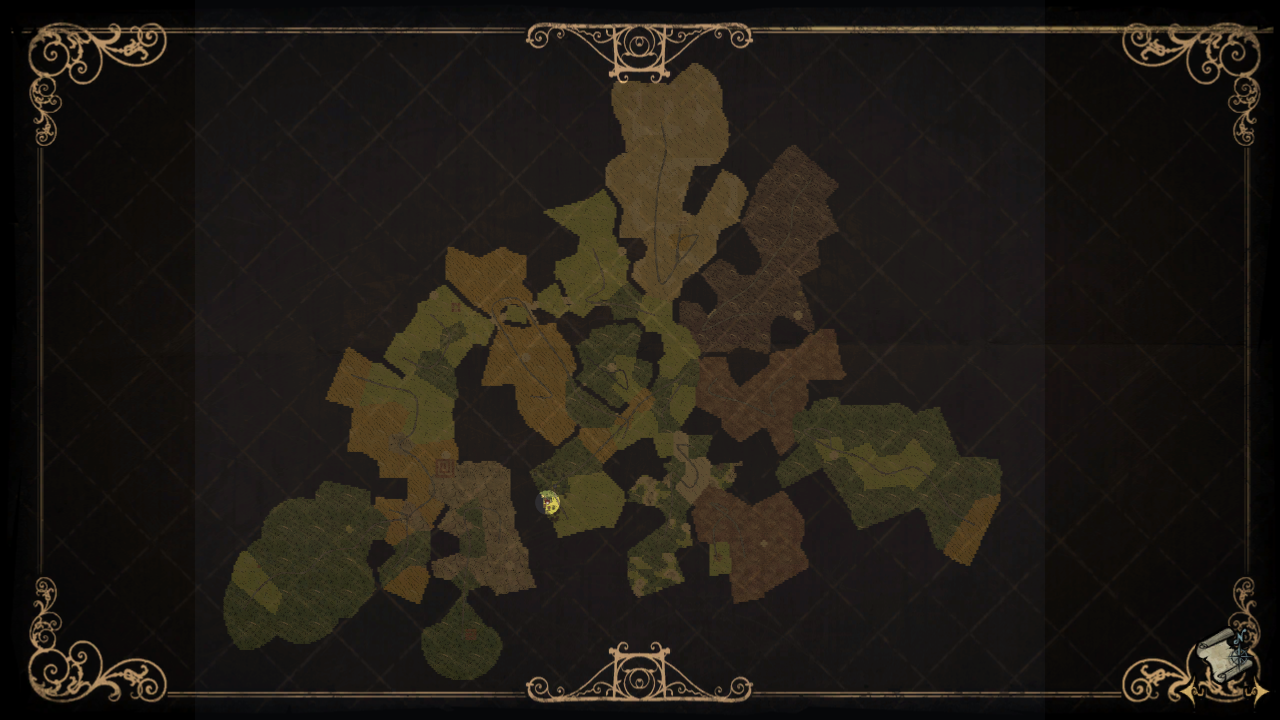
\includegraphics[width=\textwidth]{./Images/world-map}
  \caption{Example of a generated map of \ac{DST}.}
  \label{fig:world-map}
\end{figure}

\noindent As mentioned earlier, the world is procedurally generated for each game and has several different biomes that provide different kinds of resources but also dangers for the player. 
We'll present and describe these biomes later on.

The world is surrounded by water and is, in many cases, composed by several peninsulas which can be composed by one or several biomes, as can be seen in Fig. \ref{fig:world-map}.
It's also common to see the formation of lakes inside the main portion of land.

During gameplay, time will pass not only in a night and day cycle but also across seasons.
The game has four seasons (Autumn, Winter, Summer, and Spring) that present different challenges during the course of the game.
In Winter, the temperature descends a lot, while in Summer, the temperature rises, causing the player to take damage over time due to extreme temperatures.
In Spring, the commonly occurring rains will increase the character's Wetness, which will have the effects already described.
Autumn is by far the friendlier season, with mild temperatures and occasional rains, making it the perfect candidate for the starting season.

Seasons bring yet another challenge for players: giants (see Fig. \ref{fig:dst-deerclops}).
During each season, a giant (for each season there is the corresponding giant) will spawn in the vicinity of the player and will attack him.
The player can either choose to engage in a fight with the giant or try and lure him away until the giant looses interest.

A normal world will also have caves that the players can descend to, but we will not discuss them here since we won't consider them for our work.

\begin{figure}
  \centering
  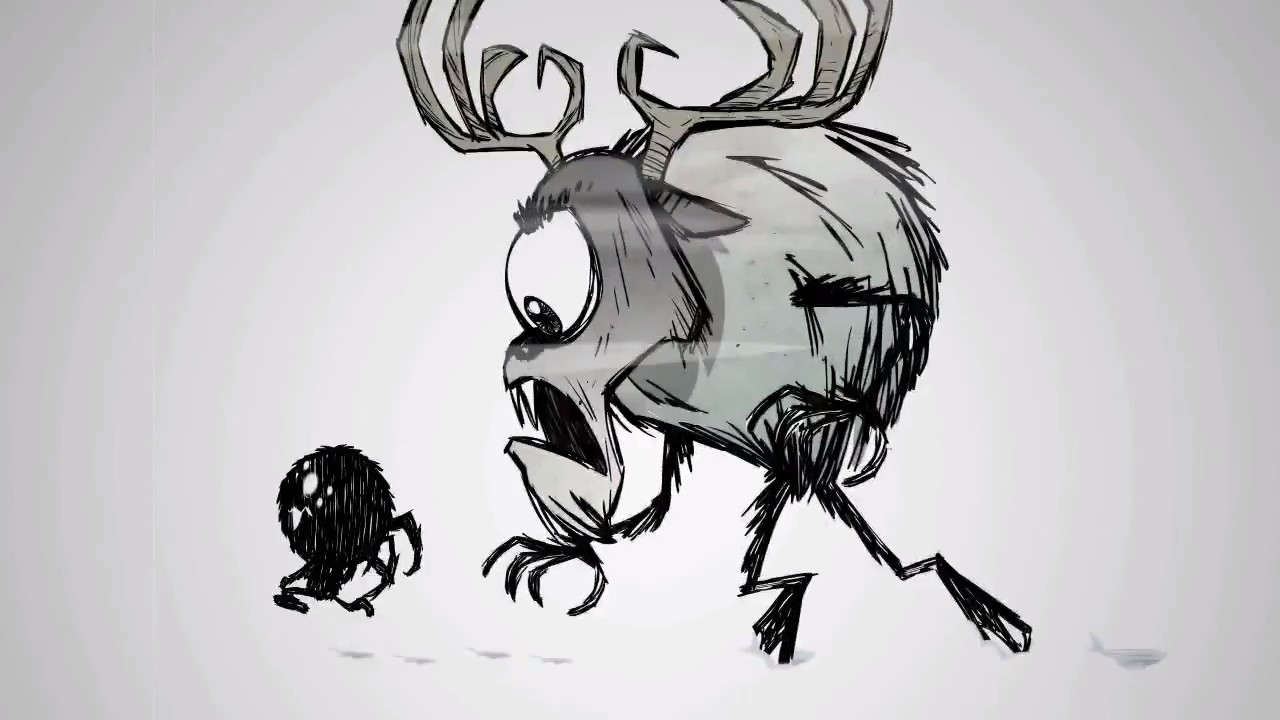
\includegraphics[width=\textwidth]{./Images/dst-deerclops}
  \caption{Deerclops, the Winter giant, chasing after Webber.}
  \label{fig:dst-deerclops}
\end{figure}

Moving on to the specifics of each biome, we'll now explore a list of all the available biomes on \ac{DST} and a brief description for each of them:

\begin{itemize}
\item \textbf{Chess} this biome has an abundance of marble (a very rare material in the game), however it is protected by aggressive mobs;
\item \textbf{Deciduous Forest} being a forest, this biome is a great source of wood but also fireflies and mushrooms;
\item \textbf{Desert} can be a good source of grass and twigs (two of the most important resources on the game) but can also be very dangerous due to the Hound mob spawn points;
\item \textbf{Forest} a very good source of wood but can also contain spiders;
\item \textbf{Grassland} one of the safest biomes where the player can find a good variety of resources;
\item \textbf{Graveyard} can contain many gold nuggets and can be hazardous free.
By digging up graves the player can collect loot but there is a chance that a Ghost may spawn and attack the player.
\item \textbf{Marsh} commonly known as Swamp, is the harshest biome in the game, everything here will try and kill the player;
\item \textbf{Mosaic} this biome typically appears only once per map, and is a mix of all other biomes with not so great resources;
\item \textbf{Savanna} the abundance of grass and mobs (passive mobs like Rabbits, Birds, and Beefaloes) make this biome the best for the player to settle.
Although it can also become a dangerous place during the Beefaloes mating season where they become aggressive;
\item \textbf{Rockyland} a barren biome that contains a lot of boulders but almost nothing else. It’s a common place for Tallbirds, an aggressive mob.
\end{itemize}

%For a complete listing of all the resources and where to find them, see Appendix B.

The knowledge of each of these biomes will differentiate good players from expert players, as it can strongly influence their success.
Players must know where to for look what they need, where to settle, places to avoid, among others.

For the remainder of this section, we'll explore the environment of \ac{DST} which we just described in a more formal way.

According to Russel and Norvig's classification of environments \cite{russell&norvig:aima}, \ac{DST} is a partially observable, multiagent, stochastic, episodic, dynamic, continuous, and known environment.

\begin{description}
	\item \textbf{Partially observable} In \ac{DST} the environment is actually fully observable through the scripts it natively provides to the modders and every entity is directly accessible to the agent. Despite this, we've decided to limit the observability of the environment to keep the agent in the same level of knowledge with the player, therefore, it will only have access to the same area as seen by the player in the screen.
	\item \textbf{Multiagent} The world may contain several players, and is therefore a multiagent environment.
	\item \textbf{Stochastic} During the game, spontaneous rains can occur, meteors can fall from the skies, and even lightning strikes can set the players crops ablaze. 
	This all happens randomly and the agent will need to act accordingly in order to survive.
	\item \textbf{Episodic} Although the world is in a continuous flow, we can consider it an episodic environment. 
	Due to the continuous passage of time, day after day and season after season, the player will have to overcome recurring problems.
    Every night the player will have to deal with darkness (which can kill the player) and every season similar challenges (Winter always presents the same challenges).
	\item \textbf{Dynamic} During the deliberation process of the agent, the environment around him can change without direct interference from it, be it through the passing of time and therefore seasons, or be it by the aggressive and passive mobs that populate the world (e.g. Moleworms search for and eat flints, one of the most valuable resources in the game)
	\item \textbf{Continuous} In \ac{DST} time passes continuously without interruptions and even actions take time to achieve, e.g. when collecting resources there is an associated animation that must be completed for the agent to effectively receive the resources.
	\item \textbf{Known} The laws that rule \ac{DST} are all known to the agent and therefore the outcome for every action is known.
\end{description}

As described above, the world in \ac{DST} isn't a trivial one and will therefore represent a strong challenge when developing an \ac{NPC}.
However, the rules that apply to each generated world may vary and can be customized.
Before starting the game, the player can tweak with a set of different options to personalize the resulting world.

Tweaks vary from very simple stuff, like increasing the rate at which hounds attack the player, to game changing stuff, like disabling all monsters in the game.
This ability to personalize the world, is crucial to creating worlds with various degrees of challenge for the players and possible \ac{NPC}s.

\section{Gameplay}

\noindent In order to survive, players must keep Health, Sanity and Hunger in check, as described before.
To achieve this, players must collect resources, craft weapons, tools, and equipments, fight, and find a home.
For the remainder of this section we'll explore, in a general view, what does a player do when playing \ac{DST}.
This will allow us to identify what sort of actions our agent will perform and group them into specific problems.
Before the end of the section, we'll have a comprehensive view of the problem which will allow us to better understand how can we solve it.

The first few days in \ac{DST} are the most crucial ones.
Players will usually collect flint and twigs, used in the construction of tools like axes and pickaxes, in order to collect logs (to build a fire) and gold nuggets (very important for prototyping new tools and weapons).
Finding food is of the utmost importance. 
Players usually rely on berries and carrots, which can be easily caught during the first days.
Collecting cut grass is also of the most importance given that the players will need to build traps in order to keep stockpiling food.

Along with all the collecting, players must explore the world, with the intent of finding a resource filled area where they will later set up a base camp.
Usually, by the end of the fifth day, players will have found a suitable place to build a base camp and will have found at least a gold nugget.

In the beginning, players will only have the knowledge to craft basic tools and equipment, e.g. axes, pickaxes, hammers, Grass Suits (armour), Straw Hats, among others, in a total of fifteen recipes.
By building a Science Machine, which will consume a gold nugget, players will be able to prototype new items, thus learning the recipes for them.
After prototyping a new item, players are able to freely craft that item, given that they have the required materials.
As the game progresses, players learn up to a total of over one hundred and fifty recipes.

\begin{figure}
  \centering
  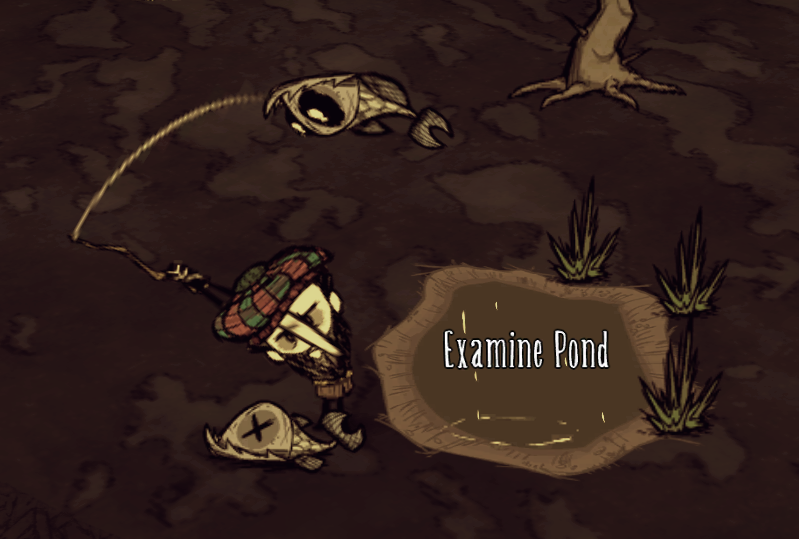
\includegraphics[width=\textwidth]{./Images/fishing}
  \caption{Wilson fishing in a pond.}
  \label{fig:fishing}
\end{figure}

As for the base camp, players tend to find places which can provide great quantities of meat since it will be the base of the players diet after the first few days.
Rabbit holes and Ponds are usually good places, as every day they spawn Rabbit and Frogs, respectively.
Additionally, ponds can be harvested with a Fishing Rod in order to collect fishes (Fig. \ref{fig:fishing}), that once cooked in a Crock Pot will provide a good Health regenerative.
Another important factor in the choosing of a base is the proximity to manure, a must have resource for the building of farms.

As the time passes and players start to have a steady supply of food items, the tendency is to start relocating other resources to make them more accessible.
Most players will dig up Grass Tufts, Sapplings, and Berry Bushes (they provide Grass, Twigs, and Berries, respectively) and plant them near the base camp, as seen in Fig. \ref{fig:basecamp-example}.
This will greatly increase a players collecting rate as all will be concentrated in an area around the players' camp, whereas the natural occurrence of such resources is usually sparse (occasionally, Berry Bushes and Grass Tufts will spawn in small clusters of nine elements near Pig Villages).
However, the relocation of Grass Tufts and Berry Bushes is usually troublesome as they require to be fertilized (using manure) in order to regrow.

\begin{figure}
  \centering
  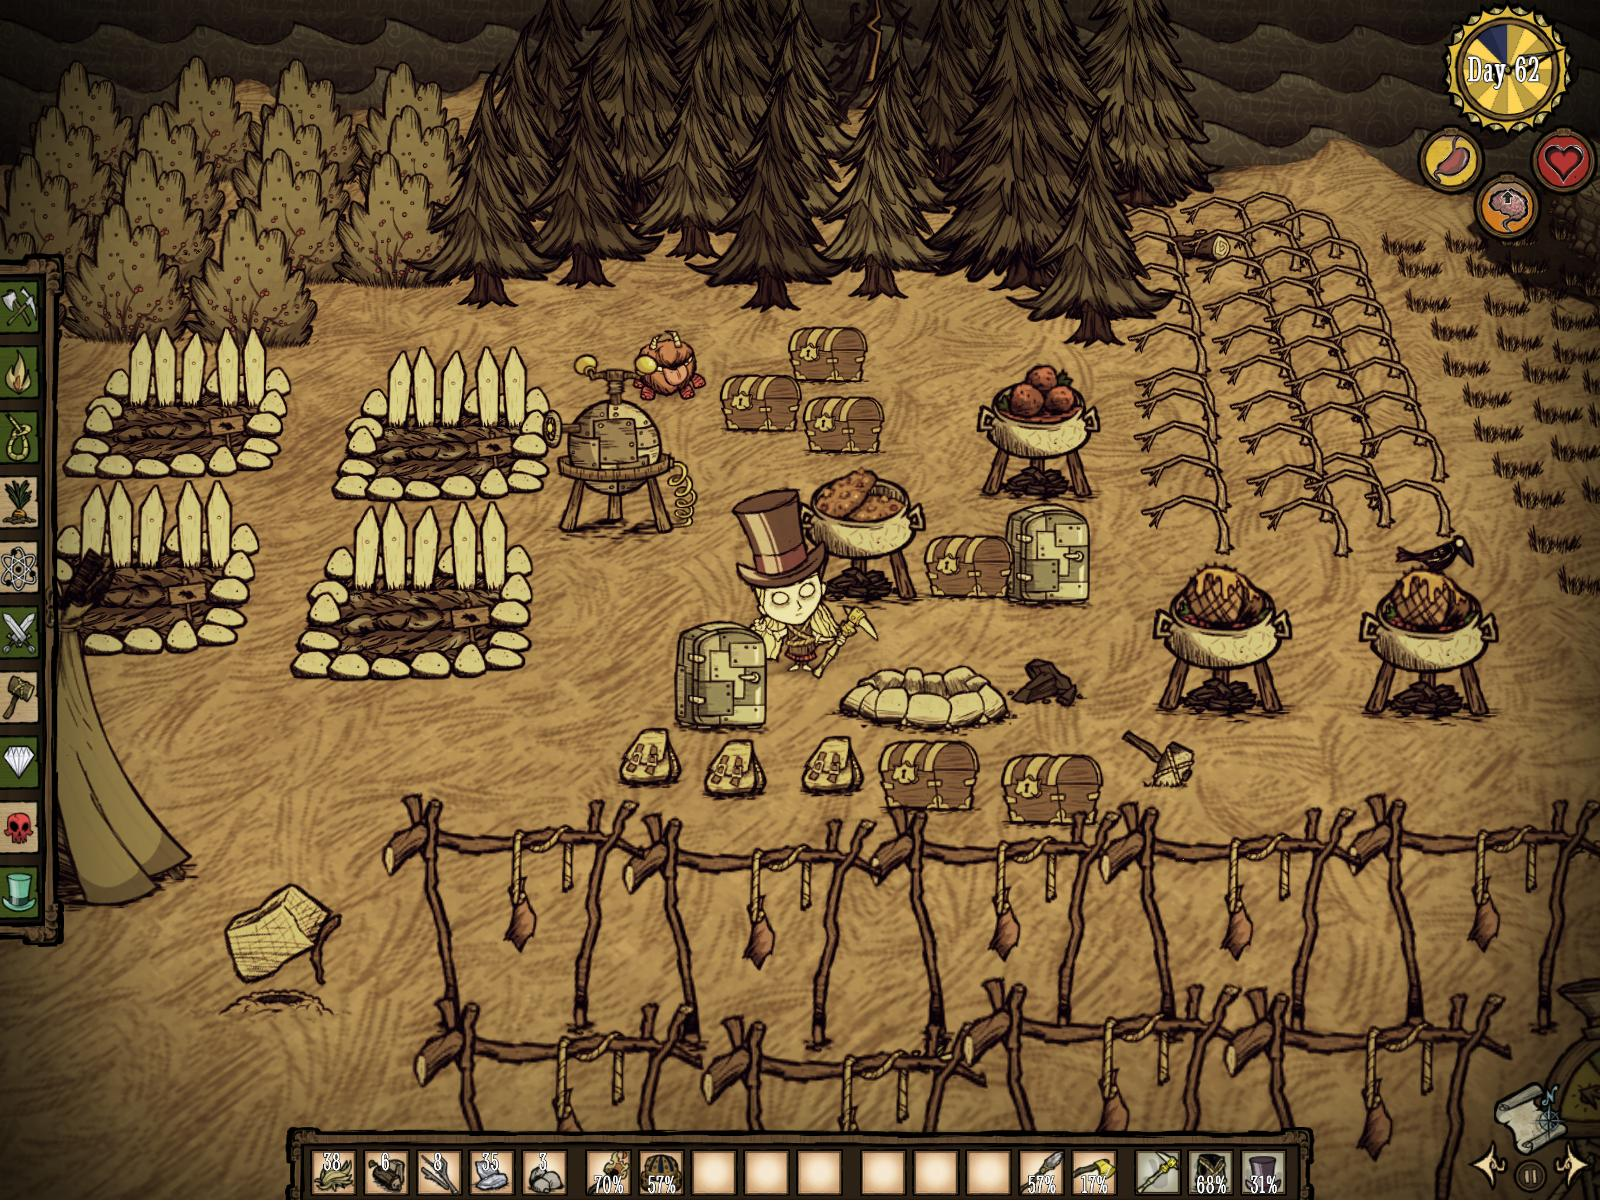
\includegraphics[width=\textwidth]{./Images/basecamp-example}
  \caption{An example of a base camp.}
  \label{fig:basecamp-example}
\end{figure}

In order to feed themselves, players use the Crock Pot to cook the food.
Crock Pots allow the elaboration of dishes that have several beneficial characteristics.
They can restore Hunger, Health and Sanity, with different dishes having different values, e.g. Fish Sticks restore a lot of Health but don't restores as much Hunger while the Meaty stew does the opposite.
For the cooking of dishes players use meats and vegetables.
The later is often obtain from farms, hence their presence in a players' base camp.

The base camp will usually be composed by a Science Machine or an Alchemy Engine (an improved version of the Science Machine), Farms, Drying Racks (used to dry meat which can them be stored for a longer period), Crock Pots, Chests (used to store items), clusters of Tress, Grass Tufts, and Saplings, and one or more Firepits.

As said before, if players stand in complete darkness for too much time, Charlie, the antagonist of the game, will attack and kill the player.
By standing next to a source of light, like a campfire, the player avoids being attacked by Charlie.

\section{Closing Remarks}

\noindent We've now thoroughly explored \ac{DST} game mechanics and frequently faced adversities.
A player's main concern is to keep the character's stats balanced throughout the game and find ways to survive the dangers each season brings.
To keep a steady supply of food and protection from the elements is as important as defending themselves from the monsters that will try to kill them.

To wrap up this chapter, bellow is a list of the core game mechanics with a small description.
This list represents a compilation of key aspects we have to take into account while making an \ac{NPC} for \ac{DST}.

\begin{description}
	\item[\textbf{Health}] \hfill \\ When it reaches zero a character dies. It can be replenished by certain items and by eating appropriate food and will be lost while fighting and when in extreme conditions of temperature.
	\item[\textbf{Hunger}] \hfill \\ Will cause a character to start losing health when it reaches zero. It will gradually decrease over time and can be increased by eating food.
    \item[\textbf{Sanity}] \hfill \\ Represents the mental state of the character. Certain conditions will cause it to decrease (e.g. fighting or standing in the dark) while others can cause it to increase (e.g. eating certain foods or being around befriended \textit{pigmen}). When near zero will provoke hallucinations that can attack the character. 
	\item[\textbf{Temperature}] \hfill \\ In cases of extreme cold or heat the character will start to lose health over time. It can be kept in check with the use of craftable items like clothes and fires.
	\item[\textbf{Wetness}] \hfill \\ As the character gets herself wet it can drop held items, food in the inventory will spoil faster, and her temperature will also decrease. The use of umbrellas and appropriate clothing will prevent the wetness level from rising.
    \item[\textbf{Darkness}] \hfill \\ When in complete darkness a character will be attacked by the darkness creature. It is important to stay near a source of light during the night.
    \item[\textbf{Fighting}] \hfill \\ Either as a means of defense or of gathering food, fighting is a core game mechanic without which survival is impossible.
\end{description}